\documentclass[11pt]{beamer}
\usetheme{default} 

\setbeamertemplate{navigation symbols}{} %gets rid of navigation symbols
\setbeamertemplate{footline}{} %gets rid of bottom navigation bars
\setbeamertemplate{footline}[page number]{} %use this for page numbers

\setbeamertemplate{footline}{%
  \raisebox{5pt}{\makebox[\paperwidth]{\hfill\makebox[10pt]{\scriptsize\insertframenumber~~}}}}

\setbeamertemplate{itemize items}[circle] %round bullet points
\setlength\parskip{10pt} % white space between paragraphs

\usepackage{wrapfig}
\usepackage{subfig}
\usepackage{setspace}
\usepackage{enumerate}
\usepackage{graphicx}
\usepackage{amsmath}
\usepackage{amsfonts}
\usepackage{amssymb}
\usepackage{amsthm}
\usepackage[UKenglish]{isodate}
\usepackage{tikz}
\usepackage{pgfplots}
\usepackage{natbib}
\usepackage{hyperref}
\hypersetup{
    colorlinks=true, 
    urlcolor=blue
}
\def\checkmark{\tikz\fill[scale=0.4](0,.35) -- (.25,0) -- (1,.7) -- (.25,.15) -- cycle;} 

% allow drawing arrows
\usetikzlibrary{arrows}
\tikzstyle{arrow}=[draw, -latex] 

% bracketing shortcuts
\newcommand{\paren}[1]{\left(#1\right)}
\newcommand{\sqbracket}[1]{\left[#1\right]}
\newcommand{\cbracket}[1]{\left\{#1\right\}}
\newcommand{\abs}[1]{\left\lvert#1\right\rvert}
\newcommand{\norm}[1]{\left\lVert#1\right\rVert}
% set up the argmin operator, argmax
\DeclareMathOperator*{\argmin}{arg\,min}
\DeclareMathOperator*{\argmax}{arg\,max}

\newcommand{\myframe}[1]{\begin{frame} \frametitle{#1}}

% New itemize environment, with spaces
\newenvironment{spaceitemize}
{ \begin{itemize}
    \setlength{\itemsep}{10pt}
    \setlength{\parskip}{0pt}
    \setlength{\parsep}{0pt}     }
{ \end{itemize}                  } 


% the preamble
\title{Day 3, Session 1: R and RStudio basics}
\author{Jessica Williams-Nguyen and Brian D. Williamson}
\institute{EPI/BIOST Bootcamp 2017}
\date{26 September 2017}

% Start the document
\begin{document}
% The title page
\begin{frame}
\titlepage
\end{frame}

% R intro
\section{The R and RStudio interfaces}
\myframe{The interface}
We interact with both R and RStudio using an interface. For R, this is the command line. For RStudio, this is the graphical user interface.

Both of these concepts deserve a bit of introduction, since familiarity with the interface makes using R and RStudio much easier!
\end{frame}
\subsection{R}
\myframe{Command line R}
The most basic form of R is from the command line (Terminal in Mac/Linux, Command Prompt in Windows). 

After installing R, typing R in the command line will open an R session:
\begin{center}
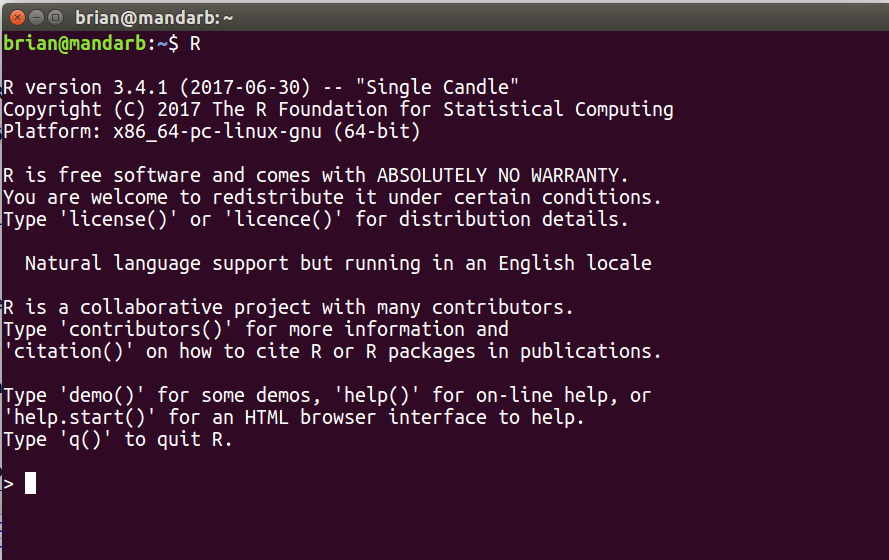
\includegraphics[width = .6\textwidth]{figs/command_line_r.png}
\end{center}

The text gives you the version number (here, 3.4.1) and some other (not necessary for our purposes) information. 
\end{frame}

\myframe{Command line R}
You also get a prompt, the \texttt{>}, where you can enter commands. 

When you first open R, you have a limited number of functions available for use. These include things like \texttt{mean()}, \texttt{median()}, and \texttt{read.table()}. 

The command line version of R is most useful (in my experience) for computing-intensive tasks. Data analyses are best done in RStudio.
\end{frame}

\subsection{RStudio}
\myframe{RStudio}
When you first open RStudio, you are met with a blank set of four \textcolor{blue}{panes}:
\begin{center}
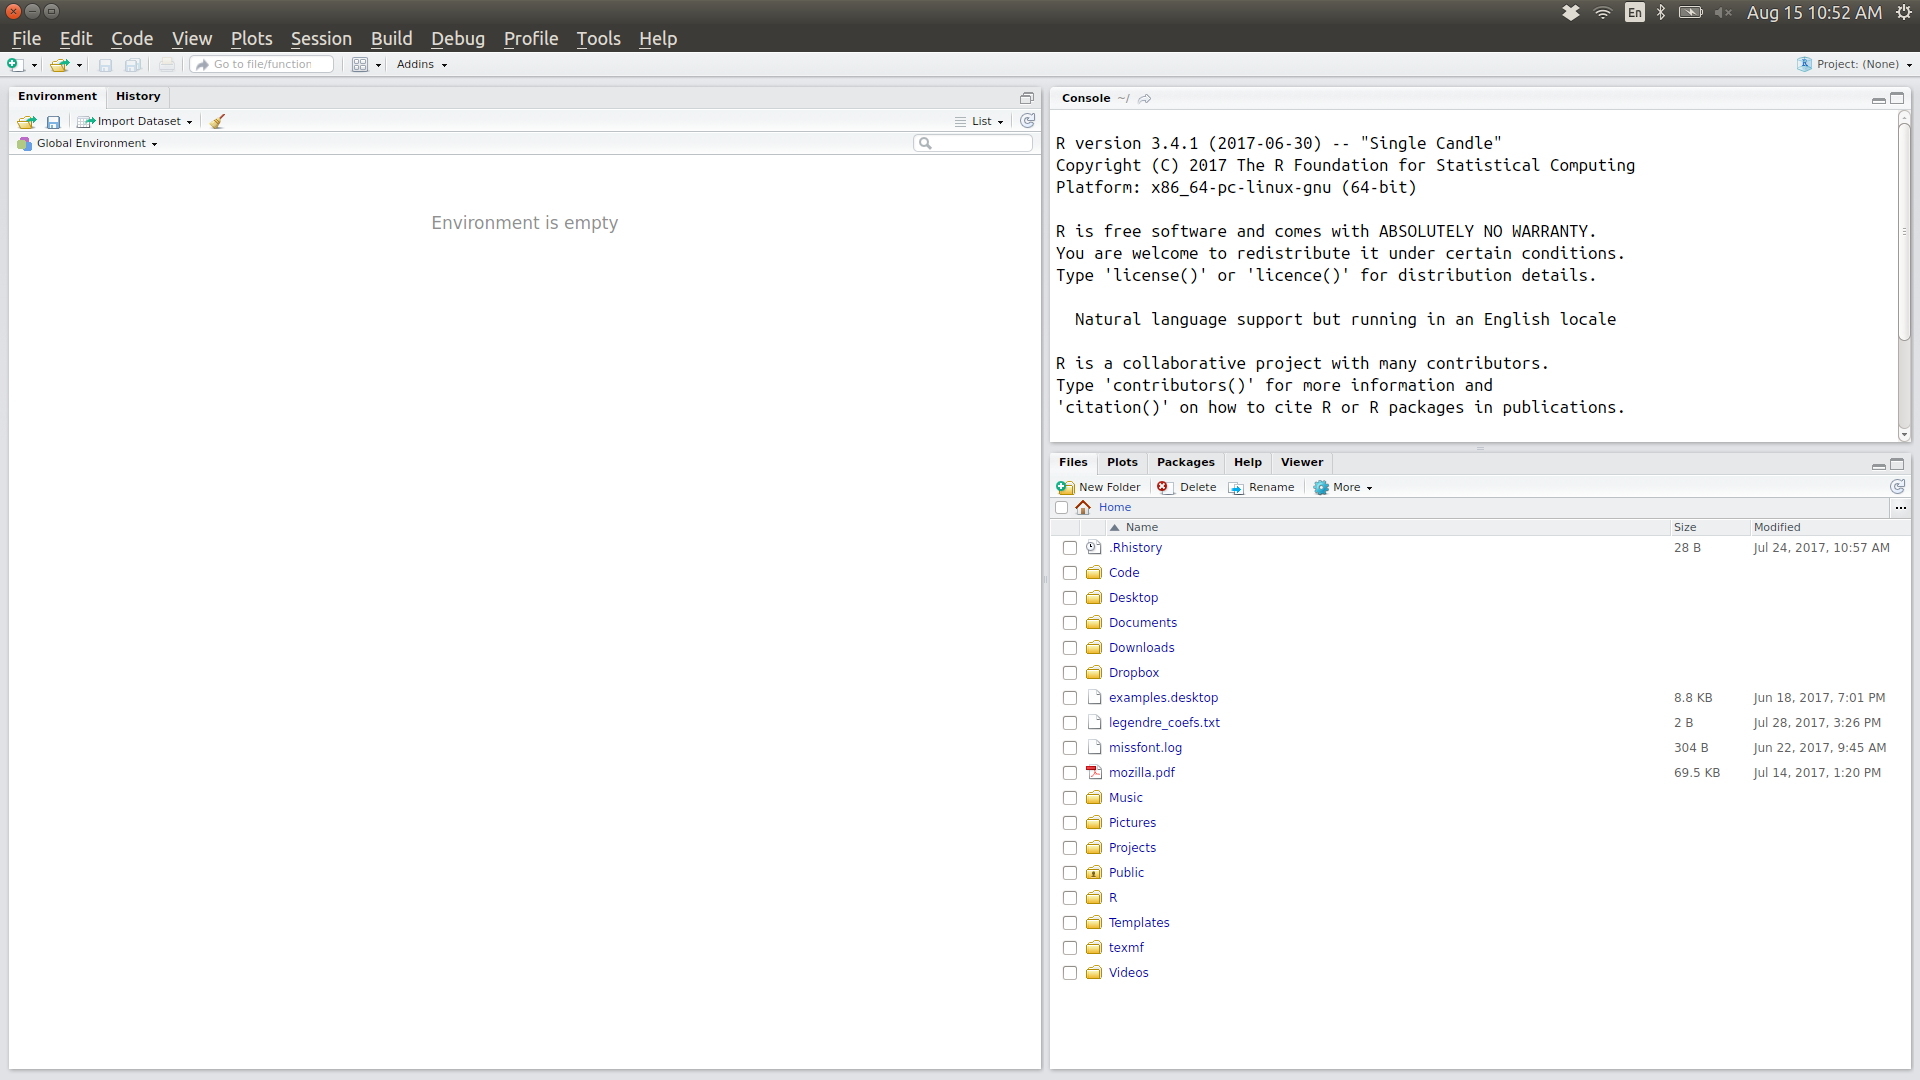
\includegraphics[width = 0.8\textwidth]{figs/rstudio.png}
\end{center}
\end{frame}

\myframe{RStudio}
You can edit pane layout under \texttt{Tools > Global Options > Pane Layout}. My preference is to have the \textcolor{blue}{source} in the upper left, \textcolor{green}{console} in the upper right, \textcolor{cyan}{environment} in the lower left, and \textcolor{purple}{viewer} in the lower right.

You'll notice that on the previous slide, there were only three panes visible: since we haven't opened or created any files to edit, the \textcolor{blue}{source} pane is not currently open.
\end{frame}

\subsubsection{The console}
\myframe{RStudio: the console}
Is it a coincidence that the screenshot has exactly the same text as we saw on the command line? No! 

The \textcolor{green}{console} performs identically to the command line. Any commands that we wish to enter go through the console, and any results that are output by these commands will appear in the console. 

\end{frame}

\begin{frame}[fragile]
\frametitle{Example: the console}
Typing \texttt{47} at the \texttt{>} symbol (from now on, called the execution line) and hitting \texttt{Enter} on the keyboard yields the following:
\begin{verbatim}
> 47
[1] 47
\end{verbatim}

Since R is a \textcolor{blue}{functional} programming language, typing \texttt{47} and hitting \texttt{Enter} is the same thing as using the \texttt{print()} function:
\begin{verbatim}
> print(47)
[1] 47
\end{verbatim}

The output is displayed as a \textcolor{green}{vector}, one of the fundamental \textcolor{cyan}{data structures} in R. The \texttt{[1]} helps to tell which element of the vector we are looking at (which is most useful if the vector spans multiple lines in the console).
\end{frame}

\myframe{Example: heights and weights}
The console is the workhorse of RStudio. If we wanted, we could work exclusively here, but then reproducibility is difficult...

Let's say we have data on the height and weight of five (imaginary) individuals. A simple way of reading the data into R is by creating two \textcolor{blue}{objects}, \texttt{ht} and \texttt{wt}, and assigning the numerical values that we have collected for each individual; in the console, type
\begin{enumerate}
\item \texttt{ht <- c(72,65,84,73,68)}, followed by hitting the \texttt{Enter} key, (creates the \texttt{ht} object)
\item \texttt{wt <- c(165,120,210,180,125)}, followed by hitting the \texttt{Enter} key (creates the \texttt{wt} object)
\end{enumerate}

Each of these commands assigns a \textcolor{green}{value} to an \textcolor{blue}{object}, using the special \texttt{<-} command. \textcolor{green}{Values} go on the right-hand side, and \textcolor{blue}{objects} go on the left.
\end{frame}

\myframe{Example: heights and weights}
Both \texttt{ht} and \texttt{wt} are also vectors! We create vectors using the \texttt{c()} function, which concatenates scalars (single numbers, or single strings like \texttt{"Hello"}) into vectors.

In words, \texttt{ht <- c(72,65,84,73,68)} means: concatenate the numbers 72, 65, 84, 73, and 68 into a vector, and assign that vector to a variable (or object) called \texttt{ht}.

Typing these commands into the console allows us to manipulate both \texttt{ht} and \texttt{wt}; in particular, they can be used as arguments into many R functions.
\end{frame}

\myframe{Example: heights and weights}
However, these objects are part of the \textcolor{red}{current} R environment: this means that we can only use them while the current session of R is open. If we exit RStudio, we will have to re-enter the two lines defining both \texttt{ht} and \texttt{wt}.

For more complicated analyses, this can lead to a lot of confusion. Also, just typing in the console can lead us to forget what steps we took to get a certain figure or table.

Organizing commands into \textcolor{blue}{scripts} allows us to save exactly what we did during a given data analysis, which makes reproducible research easy. This helps both your future self and your collaborators, so that you can share what you did!
\end{frame}

\subsubsection{The text editor}
\myframe{RStudio: the text editor (``Source'')}
The text editor (which RStudio calls the \textcolor{blue}{source}) is the second most powerful part of the IDE. This allows us to edit and save files, and to run commands directly from the text file into the console.

To create a new R script, either type \texttt{Ctrl+Shift+N} or go to \texttt{File > New > R script}. There are many other options here (most notably R markdown, which we won't cover but is incredibly useful). This brings up the source pane.

At the top of the source pane are a set of buttons (with associated keyboard shortcuts) that will save the current file, run sections of code, or run the entire document. 
\end{frame}

\begin{frame}[fragile]
\frametitle{R scripts}
R scripts are collections of R commands and comments. These are run in the console to manipulate objects and produce output.

To create a comment, type a \texttt{\#} symbol. Anything on a line following a \texttt{\#} will not be run by R.

I like to include a preamble in all of my R scripts, which gives me information on when I created the file, what it does, whether or not it takes any input or produces output, and what I have changed since I started. Here is a sample:
\fontsize{7pt}{7.2}\selectfont
\begin{verbatim}
##############################################################################################
##
## FILE: <insert file name here>.R
##
## CREATED: <insert date here> by <your name here>
##
## PURPOSE: <Give a brief description of what the code in this file is supposed to do>
##
## INPUTS: <What inputs? Where does the data come from?>
##
## OUTPUTS: <What outputs? Plot/table names and locations>
##
## UPDATES:
## DDMMYY INIT COMMENTS
## ------ ---- --------
## <date> <inits> <What did you change?>
##############################################################################################
\end{verbatim}
\end{frame}

\myframe{Running commands from R scripts}
There are many options for running commands using your R script, either in individual lines or in blocks.

You can run individual lines by placing your cursor on the line and
\begin{spaceitemize}
\item hitting the green \texttt{Run} button, or
\item hitting \texttt{Ctrl+Enter} (Windows/Linux) or \texttt{Cmd+Enter} (Mac)
\end{spaceitemize}

Similarly, you run multiple lines by highlighting all desired lines and doing one of the two options described above.
\end{frame}

\begin{frame}[fragile]
\frametitle{Example: heights and weights}
We can now enter 
\begin{verbatim}
ht <- c(72,65,84,73,68)
wt <- c(165,120,210,180,125)
\end{verbatim}
into a new R script. Saving this as \texttt{ht\_wt\_analysis.R} is a start to analyzing these data! The script now looks like:
\tiny
\begin{verbatim}
##############################################################################################
##
## FILE: ht_wt_analysis.R
##
## CREATED: 15 August 2017 by Brian Williamson
##
## PURPOSE: Teach some R basics using height and weight data on 5 imaginary individuals
##
## INPUTS: None
##
## OUTPUTS: None
##
## UPDATES:
## DDMMYY INIT COMMENTS
## ------ ---- --------
##############################################################################################

ht <- c(72,65,84,73,68)
wt <- c(165,120,210,180,125)
\end{verbatim}
\end{frame}

\subsubsection{The environment}
\myframe{RStudio: environment, history, etc.}
The basic environment pane allows us to do three things: 
\begin{spaceitemize}
\item view which objects (data sets, etc.) exist in the \textcolor{blue}{\texttt{Global Environment}}
\item view the \textcolor{green}{history} of which commands were entered in the console
\item import datasets (using the buttons on the top of the pane)
\end{spaceitemize}

The \textcolor{blue}{\texttt{Global Environment}} is where commands that are executed in the console typically live --- intermediate objects created within functions (but not returned) live within function-specific environments.

The full command history for a given session is accessed in the \texttt{History} tab; this can be cycled through in the console using the up/down arrow keys.
\end{frame}

\myframe{Example: heights and weights}
Execute the commands in \texttt{ht\_wt\_analysis.R} using one of the two options we described earlier (\texttt{Run} button or \texttt{Ctrl/Cmd+Enter}). 

The environment pane then shows that \texttt{ht} and \texttt{wt} are \texttt{Values} (not data sets since they are vectors), and the history pane shows that we have input these two lines into the console. 

\centering
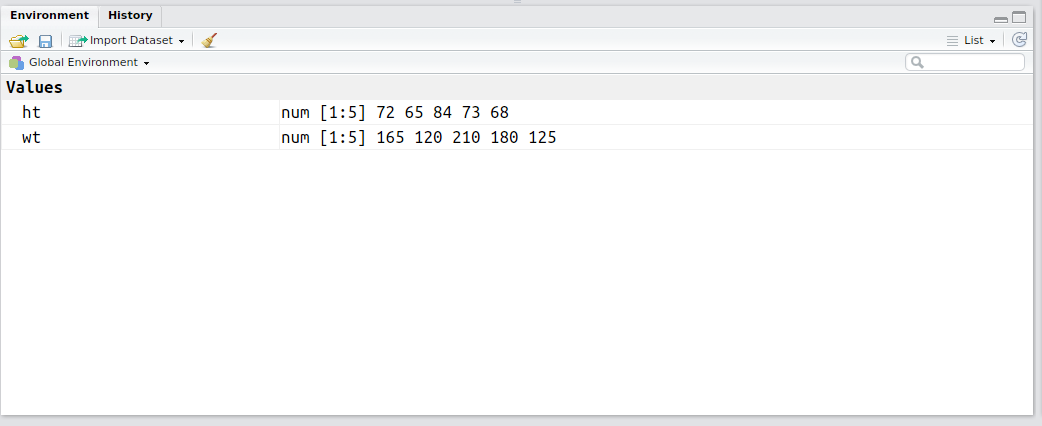
\includegraphics[width = 0.5\textwidth]{figs/environment.png}
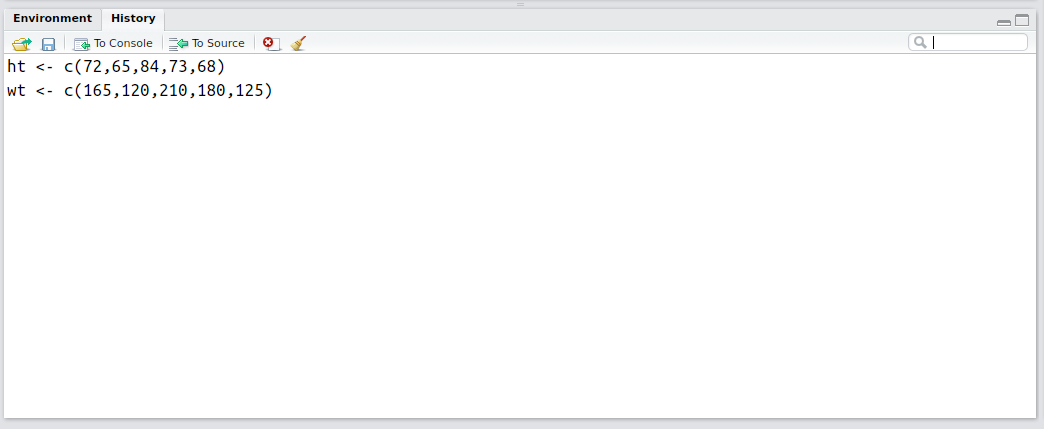
\includegraphics[width = 0.5\textwidth]{figs/history.png} 
\end{frame}

\subsubsection{The file viewer}
\myframe{RStudio: files, plot viewer, packages, help}
The final pane shows us a variety of files/plots:
\begin{spaceitemize}
\item files in the \textcolor{blue}{current working directory}
\item plots generated from executed commands
\item loaded \textcolor{green}{packages}
\item \textcolor{cyan}{help files} that we access
\end{spaceitemize}

We will cover packages and help files later on. 
\end{frame}

\myframe{The working directory}
Folders on your computer are also known as \textcolor{cyan}{directories}. These can contain data, documents, and subdirectories, among many other objects.

Your computer has a home directory, where all of your files (as the user) are stored, in different directories (e.g., \texttt{Documents}, \texttt{Pictures}, etc.). When you first log into your computer, you are in this directory.

The \textcolor{blue}{current working directory} is the directory where you are currently working. To be a bit less obtuse, consider the following example:

You have a file called \texttt{ht\_wt\_analysis.R}, located in the \texttt{Epi-Biost-Workshop} directory, which is a subdirectory of \texttt{UW}, which is a subdirectory of \texttt{Documents}, which is part of your home directory. If you double-click \texttt{ht\_wt\_analysis.R}, which opens RStudio to edit the document, your current working directory is \texttt{<your home>/Documents/UW/Epi-Biost-Workshop}.
\end{frame}

\myframe{Changing the working directory using RStudio}
Generally, when you open RStudio, your current working directory will be your home directory. This can make loading data that you have saved on your computer somewhat difficult, as we will discuss later.

One way to remedy this is to manually set your working directory using R/RStudio: either
\begin{itemize}
\item Using buttons:
\begin{enumerate}
\item In the file viewer, navigate to the folder where your dataset resides
\item Click on the \texttt{More} button (with the settings-type wheel next to it) under the file viewer tab
\item Click \texttt{Set as working directory} 
\end{enumerate}
\item Using code:
\begin{enumerate}
\item Find the path to the folder where your data resides (e.g., \texttt{/home/brian/Documents/UW/Epi-Biost-Workshop})
\item Place the code \texttt{setwd("<path to your data>")} in your R script, or enter it at the command line
\end{enumerate}
\end{itemize}
\end{frame}


\section{Introduction to R programming}
\myframe{Introduction to R programming}
We have already seen some examples of R programming: in the heights and weights example, we learned about the special \texttt{<-} command, which assigns a value to an object; and we learned about the \texttt{c()} command, which creates a vector. 

These commands relate \textcolor{blue}{functions} to \textcolor{green}{objects} --- both of these are fundamental concepts in R programming.
\end{frame}

\myframe{Functions}
R functions take in \textcolor{blue}{arguments} and return \textcolor{green}{values}. A function is accessed by typing its name, followed by an open and closed set of parentheses: e.g., \texttt{quantile()}, a function to compute desired sample quantiles.

\textcolor{blue}{Arguments} to functions go between the parentheses, and are separated by columns. You specify which object corresponds to which argument using \texttt{=}, e.g. \texttt{quantile(x = ht, probs = 0.5)} returns the median value of the \texttt{ht} object.

\textcolor{green}{Values} are returned by functions, and are generally either a combination of objects, plots, and printout. The value of the result of entering \texttt{quantile(x = ht, probs = 0.5)} into the console is a vector containing the number 72.
\end{frame}

\myframe{Objects}
R objects are (basically) the result of calling functions. However, there are two general ways this can be done:
\begin{spaceitemize}
\item \textcolor{blue}{loading data} (e.g., from a text or .csv file)
\item \textcolor{green}{manipulating another object} using a function
\end{spaceitemize}

Both \texttt{ht} and \texttt{wt} are objects; we created them by manipulating raw numbers using the \texttt{c()} function.
\end{frame}

% Accessing and manipulating data
\section{Accessing and manipulating data}
\myframe{Loading data}

\end{frame}

\myframe{Saving data}

\end{frame}

\myframe{Manipulating data}

\end{frame}

\section{R packages}
\myframe{R packages}

\end{frame}

\end{document}